\section{Public Perception of Equity}
In order to understand the public's perception of equity (via our proposed definition) and its comparison to equality in different real life scenarios, we conducted surveys on Amazon Mechanical Turk in the vein of \cite{saxena2019fairness}.

\subsection{Experimental Setup}
We recruited 150 workers by showing them four different real life scenarios. In each scenario, we proposed two fairness solutions: one based on equity and one based on equality/parity. For each scenario, we asked workers to rate how fair they think each solution is on a scale of zero to four. At the end of each scenario, we asked workers to select their preferred fairness solution for each scenario. We asked workers to provide written justification for their responses. In addition, we had a ``sanity check'' question at the end of our survey to discover and remove workers behaving randomly. The screenshot from our questionnaire is included in the Appendixes section for more detailed information.

% Fairness definitions are context sensitive, and the purpose of our experiment is to illuminate scenarios when one is preferred. Thus, we incorporate different situations in our survey and observe how people would react in choosing the appropriate solution that follows a certain fairness definition. It is worth mentioning that finding a universal fairness definition that is appropriate in all the possible situations is challenging and almost impossible. This is because defining fairness is still an open question in philosophy let alone computer science which fairly recently has geared focus toward fairness. Our goal is to propose a new definition that would be appropriate and preferred to use in certain situations over other definitions. By no means we claim that our definition is universal, but we claim that our definition can be preferable over others in some situations. This can also be observed in the results below.

A summary of the scenarios are as follows. Note that the experimental results follow the same numbering convention as listed below.
\begin{itemize}
    \item Scenario 1 (Equality vs Equity): We asked workers to rate pictures of equity and equality in Figure~\ref{motivation} and chose their preferred picture.
    \item Scenario 2 (School Loan): Workers rate loan distribution mechanisms. One is based on equity, which considers each student's past history of receiving a scholarship (equity). Another simply proposes to equally distribute the loan among all the students (parity).
    \item Scenario 3 (Government Subsidized Housing):  We asked respondents to rate the government subsidized housing distribution systems proposed in the survey---one based on equity considering how houses were historically distributed across different races (equity). The other proposes to equally distribute houses across different racial categories (parity).
    \item Scenario 4 (College Admission): We asked respondents to rate college admission systems---one based on equity considering if the student is a first generation college student (equity). The other equally admits students from first generation and non-first generation backgrounds (parity).
\end{itemize}
\subsection{Results}
%maybe I can also have a table to summarize the important results in it as well????????
After gathering and analyzing responses from mechanical turk workers, we observed that there are some cases in which our notion of fairness is strongly preferred by a large margin, and some other cases where preference is given to the parity notion. Fairness is subjective and different people may have different takes on what would be a fair solution to a particular case. That is the main reason why we introduce this notion as not only in some scenarios our definition will be over-preferred but also in some non-preferred scenarios it will get some preference from certain groups of people.

The statistics of ratings for each of the 4 scenarios is shown in Figure~\ref{mturk_violin}. In addition, Table~\ref{votes_stats} depicts the number of mechanical turk workers who preferred a certain solution following a fairness definition in each of the scenarios. Similar to findings in \cite{saxena2019fairness}, we also observed the support for the principle of affirmative action in our experiments which relates to our notion. From the results it is evident that strong preference is given to our notion introduced in this paper for scenarios 1 and 2, and despite the fact that scenarios 3 and 4 are not over-preferred for our notion, there are still considerable number of people who gave preference to our notion in these scenarios. All the justifications written down by the respondents were analyzed. For each preference recorded in this paper, respondents gave justifications that cover a wide range of perspectives. The dataset can be found in \footnotemark[\getrefnumber{projecturl}].

\begin{figure}
\centering
    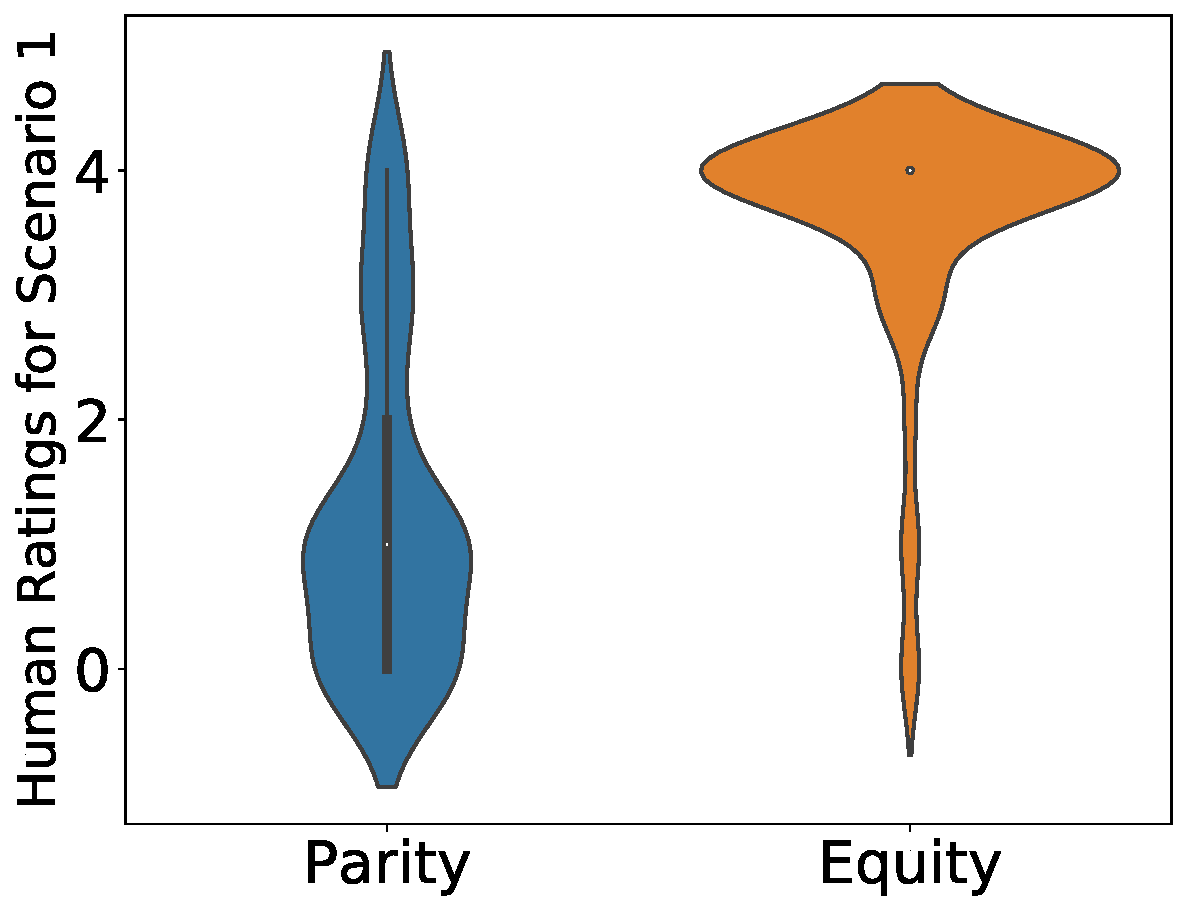
\includegraphics[width=0.23\textwidth]{images/finalQ1.pdf}
     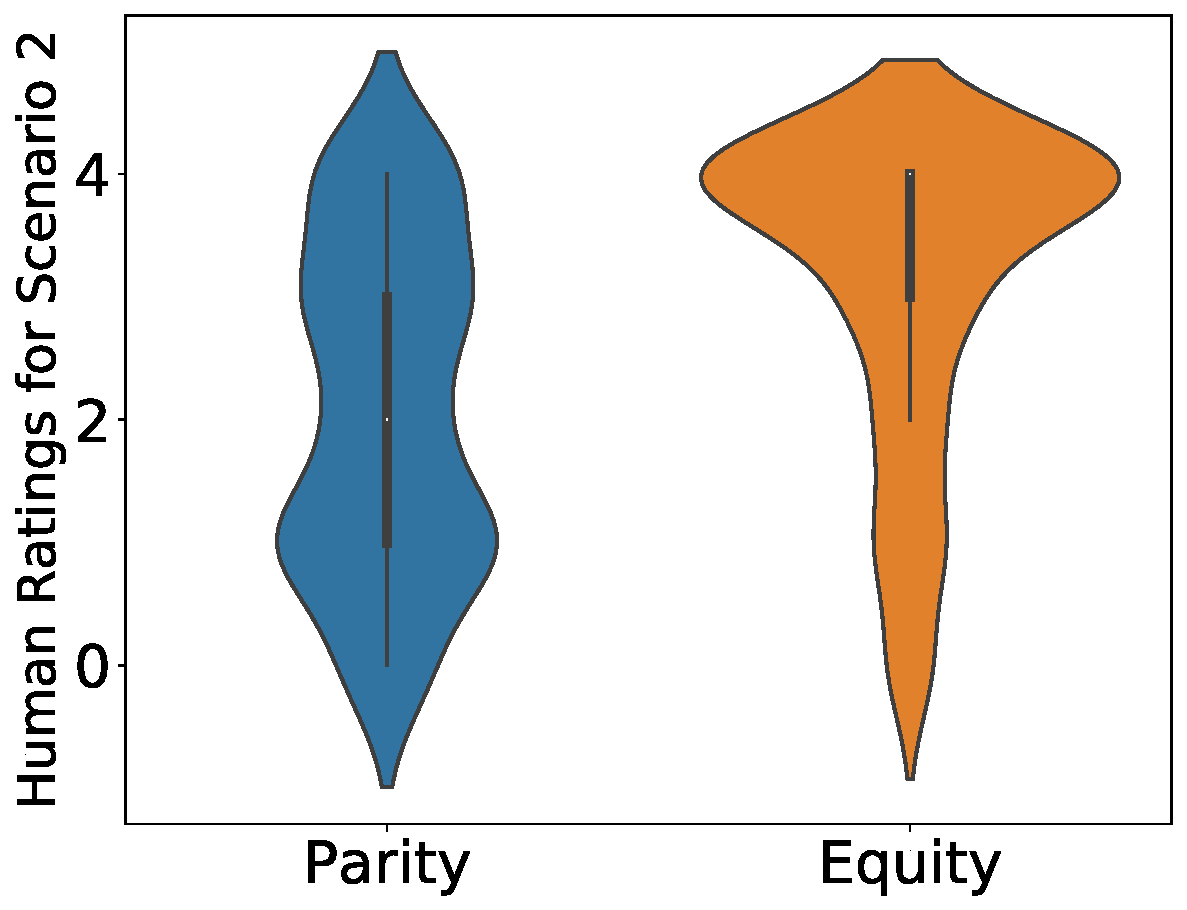
\includegraphics[width=0.23\textwidth]{images/finalQ2.pdf}
      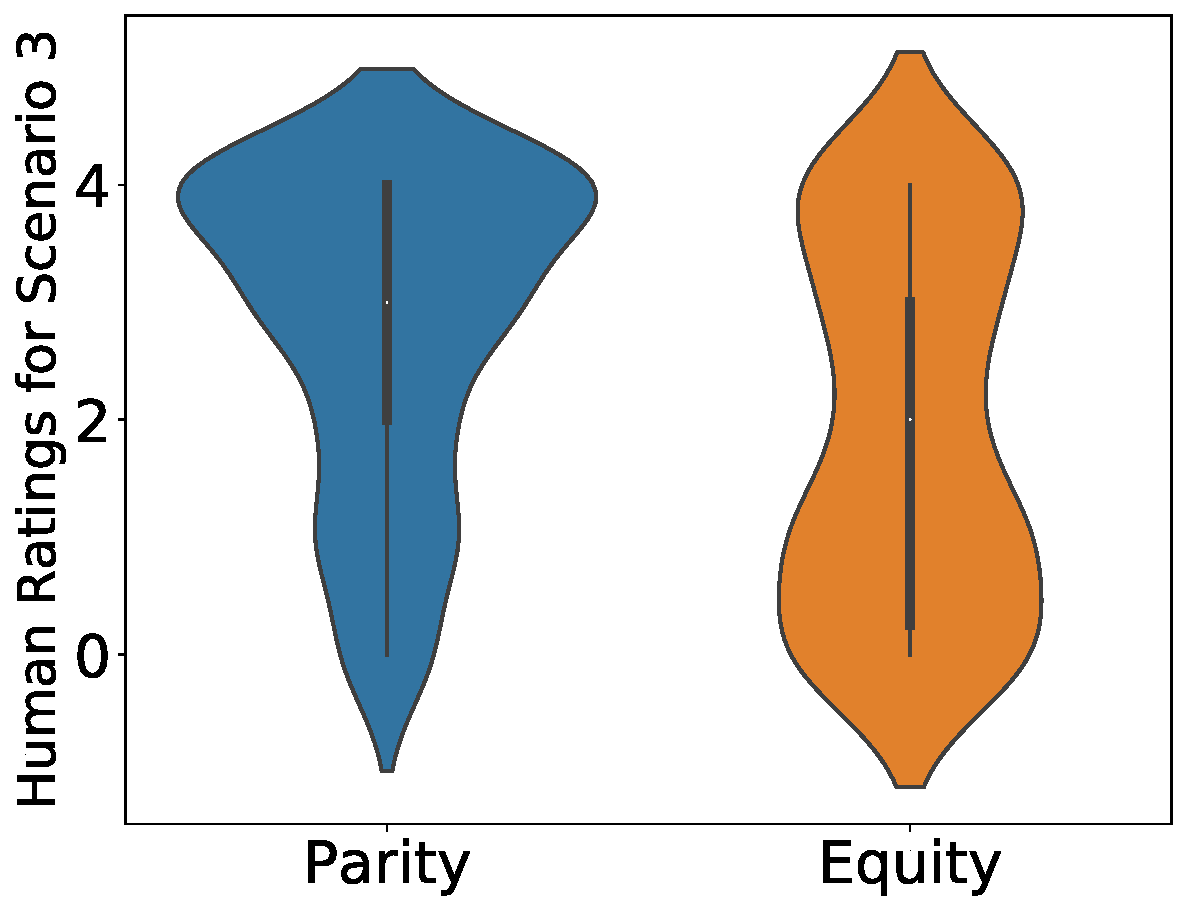
\includegraphics[width=0.23\textwidth]{images/finalQ3.pdf}
       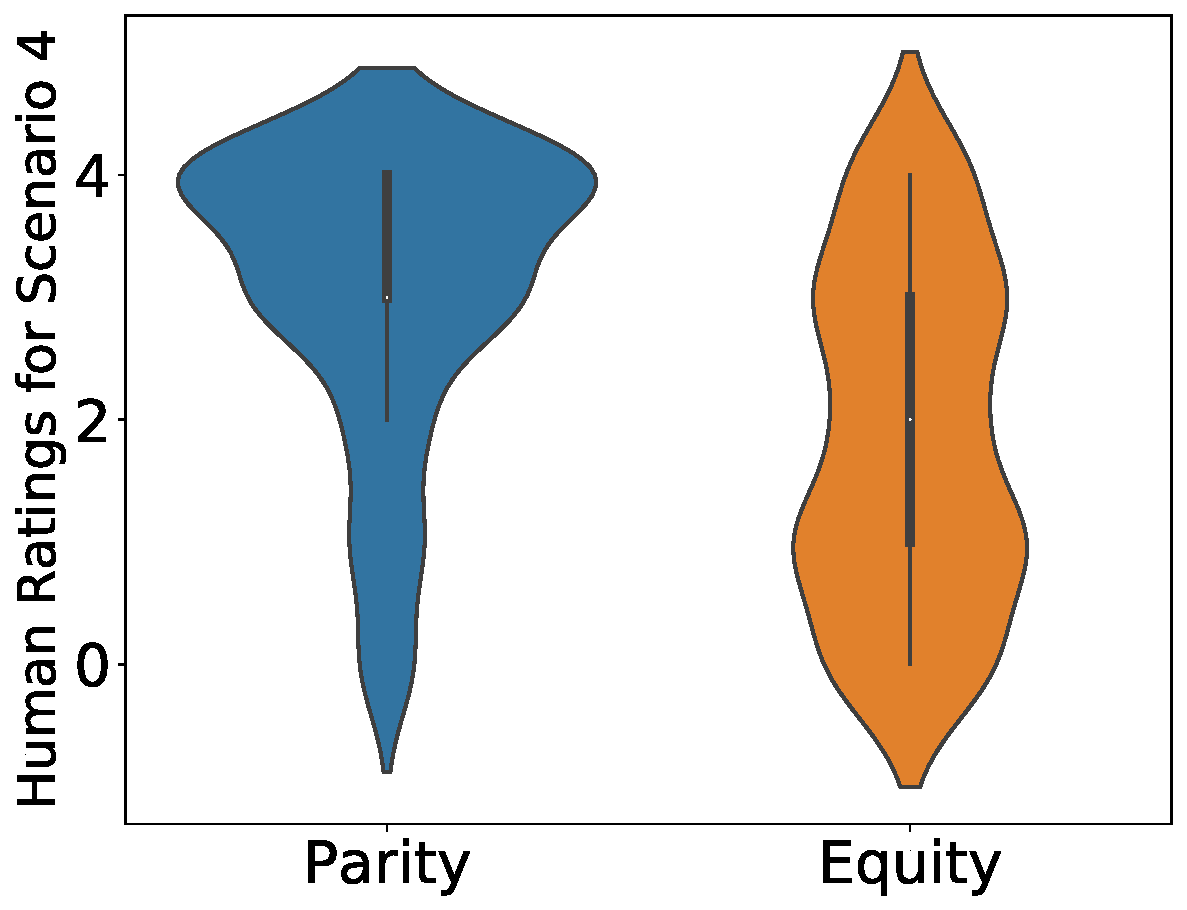
\includegraphics[width=0.23\textwidth]{images/finalQ4.pdf}
    \caption{Human ratings of equity and parity notions of fairness in different scenarios.}
    \label{mturk_violin}
\end{figure}


\begin{table}
%\centering
\begin{tabular}{ p{0.3cm} p{1.4cm} p{1.4cm} p{1.4cm} p{1.4cm}}
 \toprule
& \textbf{Scenario 1} & \textbf{Scenario 2} &\textbf{Scenario 3}&\textbf{Scenario 4}\\
 \midrule
 \parbox[t]{2mm}{\multirow{1}{*}{\rotatebox[origin=c]{90}{Equity}}}
 &\textbf{134} & \textbf{115} &59 &44\\[15pt]
 \midrule
 \parbox[t]{2mm}{\multirow{1}{*}{\rotatebox[origin=c]{90}{Parity}}} &
   16&35&\textbf{91}&\textbf{106}\\[15pt]
 \bottomrule
\end{tabular}
\caption{Number of people preferring solutions provided by the equity vs solutions provided by the parity notions of fairness in different scenarios.}
\label{votes_stats}
\end{table}


